\documentclass[conference]{IEEEtran}
\IEEEoverridecommandlockouts
% The preceding line is only needed to identify funding in the first footnote. If that is unneeded, please comment it out.
\usepackage{cite}
\usepackage{amsmath,amssymb,amsfonts}
\usepackage{algorithmic}
\usepackage{graphicx}
\usepackage{textcomp}
\usepackage{xcolor}
\def\BibTeX{{\rm B\kern-.05em{\sc i\kern-.025em b}\kern-.08em
    T\kern-.1667em\lower.7ex\hbox{E}\kern-.125emX}}
\begin{document}

\title{Triple Generative Adversarial Nets
}

\author{\IEEEauthorblockN{1\textsuperscript{st} Kaiqi Wang \ 16337233}
\IEEEauthorblockA{\textit{School of Data and Computer Sci.} \\
Sun Yat-sen University, Guangzhou, 510275, China \\
wangkq3@mail2.sysu.edu.cn}
}

%\author{\IEEEauthorblockN{1\textsuperscript{st} Chongxuan Li}
%\IEEEauthorblockA{\textit{Dept. of Comp. Sci \& Tech.} \\
%Tsinghua University, Beijing, 100084, China \\
%licx14@mails.tsinghua.edu.cn}
%\and
%\IEEEauthorblockN{2\textsuperscript{nd} Kun Xu}
%\IEEEauthorblockA{\textit{TNList Lab} \\
%Tsinghua University, Beijing, 100084, China \\
%xu-k16@mails.tsinghua.edu.cn}
%\and
%\IEEEauthorblockN{3\textsuperscript{rd} Jun Zhu}
%\IEEEauthorblockA{\textit{State Key Lab of Intell. Tech. \& Sys.} \\
%Tsinghua University, Beijing, 100084, China \\
%dcszj@mail.tsinghua.edu.cn}
%\and
%\IEEEauthorblockN{4\textsuperscript{th} Bo Zhang}
%\IEEEauthorblockA{\textit{Center for Bio-Inspired Computing Research} \\
%Tsinghua University, Beijing, 100084, China \\
%dcszb@mail.tsinghua.edu.cn}
%}

\maketitle

\begin{abstract}
Omitted.
\end{abstract}

\begin{IEEEkeywords}
Omitted.
\end{IEEEkeywords}

\section{Introduction}
Omitted.

\section{Related Work}
Omitted.

\section{Method}

\subsection{Problem Definition}

Given partially labeled dataset with $x$ denoting the input data and $y$ denoting the output label. Our goal is to learn 2 functions $G : x \rightarrow y$ to predict the labels $y$ for unlabeled data as well as $D : (x, y) \rightarrow \{0, 1\}$ to generate new samples $x$ conditioned on $y$. 

In our setting, as the label information $y$ is incomplete (thus uncertain), our density model should characterize the uncertainty of both $x$ and $y$, therefore a joint distribution $p(x, y)$ of input-label pairs.

A straightforward application of the two-player GAN is infeasible because of the missing values on $y$. We build our game-theoretic objective based on the insight that the joint distribution can be factorized in two ways, namely, $p(x, y) = p(x)p(y|x)$ and $p(x, y) = p(y)p(x|y)$, and that the the conditional distributions $p(y|x)$ and $p(x|y)$ are of interest for classification and class-conditional generation, respectively. To jointly estimate these conditional generator network, we define a single discriminator network which has the sole role of distinguishing whether a sample is from the true data distribution or the models. Hence, we naturally extend GANs to Triple-GAN, a three-player game to characterize the process of classification and class-conditional generation in SSL, as detailed below. 

We consider GANs as a semi-supervised learning model, because it uses a small amount of labeled data together with a large amount of unlabeled data. % In this case, we can get unlabeled data from model $G$ and label them by model $C$, then we can use labeled data and generated data to train model $D$. 

\subsection{Overview}

Triple-GAN consists of three components: (1) a classifier $C$ that (approximately) characterizes the conditional distribution $p_c(y|x) \approx p(y|x)$; (2) a class-conditional generator $G$ that (approximately) characterizes the conditional distribution in the other direction $p_g(x|y) \approx p(x|y)$; and (3) a discriminator $D$ that distinguishes whether a pair of data $(x, y)$ comes from the true distribution $p(x, y)$. All the components are parameterized as neural networks. Our desired equilibrium is that the joint distributions defined by the classifier and the generator both converge to the true data distribution. To this end, we design a game with compatible utilities for the three players as follows. 

The detailed structure of the Triple-GANs is shown in Figure \ref{f4}. $X_t, Y_t$ denotes labeled images and their corresponding labels, $X_c$ denotes unlabeled images, and $Z$ denotes noise vector uniformly distributed in $[0, 1]$. $p_g, p_c$ and $p$ are the distributions defined by the generator, classifier and true data generating process, respectively. The input images are $N \times N$ RGB images $X_t \in \mathbb{R}^{N \times N \times 3}$ and the input labels are $Y_t$. We also have unlabeled images which are $N \times N$ RGB images $X_c \in \mathbb{R}^{N \times N \times 3}$. 

\begin{figure}
\centering
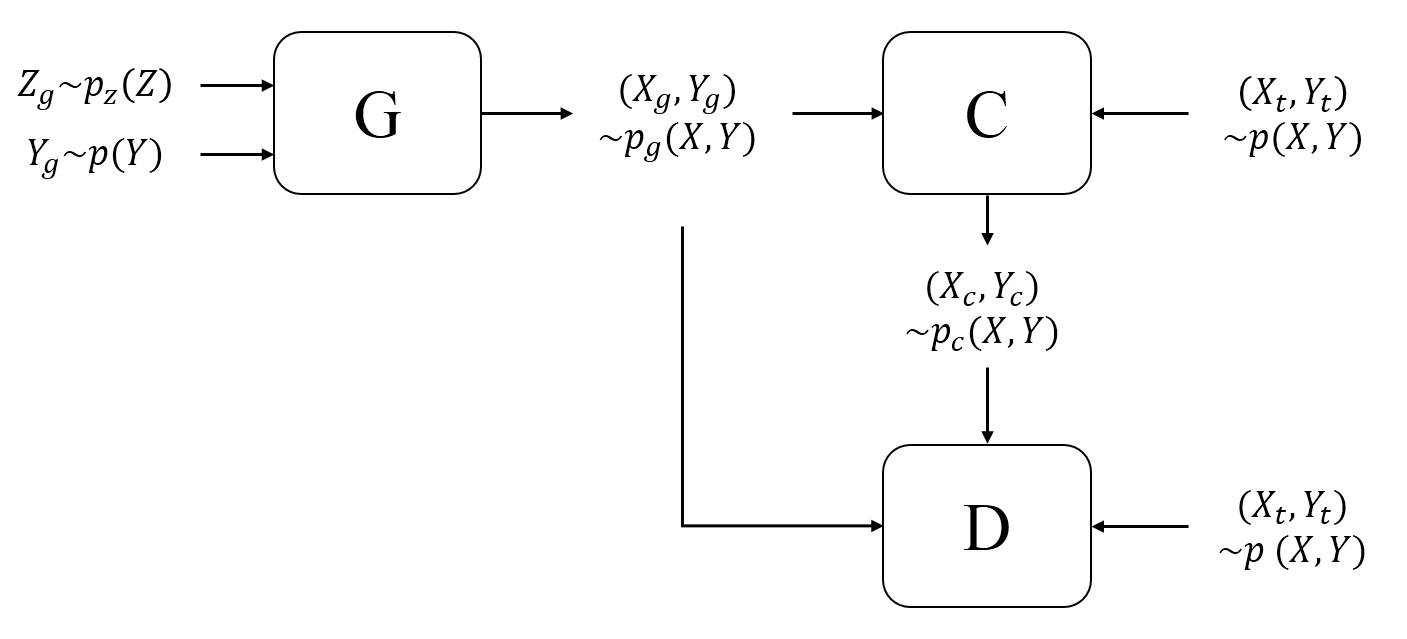
\includegraphics[scale=0.35]{pics/4.png}
\caption{A detailed structure of Triple-GANs.}
\label{f4}
\end{figure}

We make the mild assumption that the samples from both $p(x)$ and $p(y)$ can be easily obtained. In the game, after a sample $x$ is drawn from $p(x)$, $C$ produces a pseudo label $y$ given $x$ followingthe conditional distribution $p_c(y|x)$. Similarly, a pseudo input-label pair can be sampled from $G$ by first drawing $y \sim p(y)$ and then drawing $x|y  \sim  p_g(x|y)$; hence from the joint distribution $p_g(x, y) = p(y) p_g(x|y)$. Similaryly, a pseudo input-label pair can be sampled from $G$ by first drawing $y \sim p(y)$ and then drawing $x|y \sim p_g(x|y)$ ; hence from the joint distribution $p_g(x, y) = p(y) p_g(x|y)$. For $p_g(x|y)$, we assume that $x$ is transformed by the latent style variables $z$ given the label $y$, namely, $x = G(y, z), x \sim p_z(z)$, where $p_z(z)$ is a simple distribution (e.g., uniform or standard normal). Then, the pseudo input-label pairs $(x, y)$ generated by both $C$ and $G$ are sent to the single discriminator $D$ for judgement. $D$ can also access the input-label pairs from the true data distribution as positive samples. 

We refer the utilities in the process as adversarial losses, which can be formulated as a minimax game:
\begin{equation}
\begin{aligned}
\min_{C, G} & \max_{D} U(C, G, D) = E_{(x, y) \sim p(x, y)}[\log{D(x, y)}] \\
&+ \alpha E_{(x, y) \sim p_c(x, y)}[\log{1 - D(x, y)}] \\
&+ (1-\alpha) E_{(x,y) \sim p_g(x,y)}[\log(1 - D(G(y,z), y))]
\end{aligned}
\label{eq1}
\end{equation}
where $\alpha \in (0,1)$ is a constant that controls the relative importance of generation and classification and we focus on the balance case by fixing it as 1/2 throughout the paper. 

The game defined in Eqn.\ref{eq1} archieves its equilibrium if and only if $p(x, y) = (1 - \alpha) p_g(x, y) + \alpha p_c(x, y)$. The equilibrium indicates that if one of $C$ and $G$ tends to the data distribution, the other will also go towards the data distribution, which addresses the competing problem. However, unforunately, it cannot guarantee that $p(x, y) = p_g(x, y) = p_c(x, y)$ is the unique global optimum, which is not desirable. To address this problem, we introduce the standard supervised loss (i.e., cross-entropy loss) to $C$, $R_L = E_{(x,y) \sim p(x,y)}[-\log p_c(y|x)]$, which is equivalent to the KL-divergence between $p_c(x, y)$ and $p(x, y)$. Consequently, we define the game as:

\begin{equation}
\begin{aligned}
\min_{C, G} & \max_{D} \tilde{U}(C, G, D) = E_{(x, y) \sim p(x, y)}[\log{D(x, y)}] \\
&+ \alpha E_{(x, y) \sim p_c(x, y)}[\log{1 - D(x, y)}] \\
&+ (1-\alpha) E_{(x,y) \sim p_g(x,y)}[\log(1 - D(G(y,z), y))] + R_L
\end{aligned}
\label{eq2}
\end{equation}

It will be proven that the game with utilities $\tilde{U}$ has the unique global optimum for $C$ and $G$. 

\subsection{Objective Function}

\subsubsection{Generator}

\begin{figure}
\centering
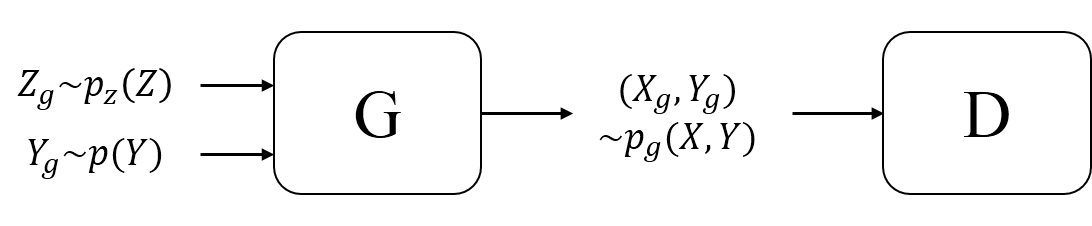
\includegraphics[scale=0.35]{pics/3.png}
\caption{The procedure of training generator: fix discriminator $D$. Generator $G$ generates and labels images and sends to discriminator $D$. Discriminator $D$ judges whether these labels are curresponding to the images. Generator $G$ gets the feedback and update its model. }
\label{f3}
\end{figure}

Generator $G$ generates as well as labels images, and sends them to the discriminator. Figure \ref{f3} illustrates the procedure of training generator. Only discriminator's response will affect generator's parameters. Hence, we can write a cross-entropy loss function,

\begin{equation}
\nabla_{\theta_g} \left[\frac{1 - \alpha}{m_g} \sum\limits_{(x_g, y_g)} \log(1 - D(x_g, y_g))\right]
\label{eq3}
\end{equation}

where $\theta_g$ denotes learning rate. 

\subsubsection{Classifier}

\begin{figure}
\centering

\includegraphics[scale=0.35]{pics/2.png}
\caption{The procedure of training classifier: fix discriminator $D$ and generator $G$. Classifier $C$ accepts true labeled images and generated images and sends to discriminator $D$. Discriminator $D$ judges whether these labels are curresponding to the images. Classifier $C$ gets the feedback and tries to improve its classification accuracy to let discriminator accept its verdict.}
\label{f2}
\end{figure}

Classifier $C$ accepts true labeled images as well as generated images, and sends them to the discriminator. And our goal is to fool discriminator. Figure \ref{f2} illustrates the procedure of training classifier. Hence, we can write a cross-entropy loss function:

\begin{equation}
\nabla_{\theta_c} \left[ \frac{\alpha}{m_c} \sum\limits_{(x_c, y_c)} p_c(y_c|x_c) \log(1 - D(x_c, y_c)) \right]
\label{eq4}
\end{equation}

\subsubsection{Discriminator}

\begin{figure}
\centering
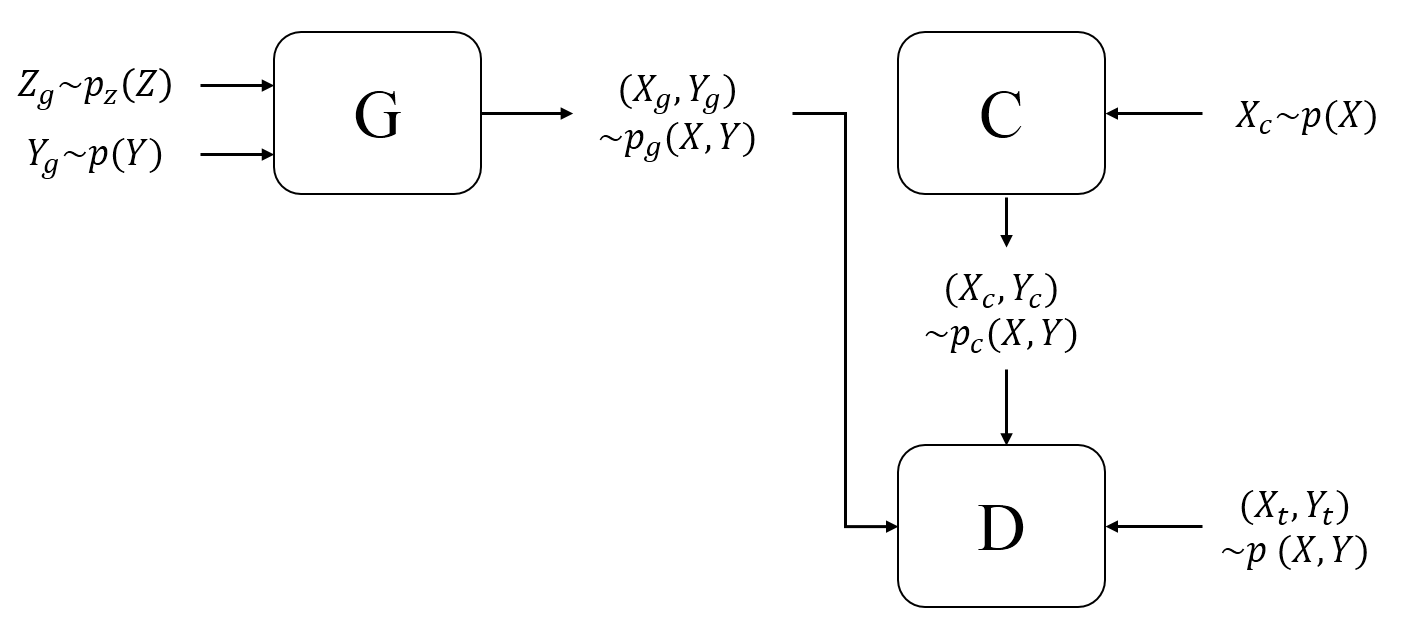
\includegraphics[scale=0.35]{pics/1.png}
\caption{The procedure of training discriminator: fix generator $G$ and classifier $C$. Discriminator $D$ accepts true images with true labels from true data, generated images with generated labels from generator $G$, and true/generated images with generated labels from classifier $C$. Discriminator $D$ gets the source of images and labels, and updates the parameters.}
\label{f1}
\end{figure}

Discriminator $D$ accepts true images with true labels from true data, generated images with generated labels from generator $G$, and true/generated images with generated labels from classifier $C$. Figure \ref{f1} illustrates the procedure of training discriminator. Hence, we can write a cross-entropy loss function:

\begin{equation}
\begin{aligned}
\nabla_{\theta_d} [ & \frac{1}{m_d} (\sum\limits_{(x_d, y_d)} \log D(x_d,y_d)) \\ 
& + \frac{\alpha}{m_c} \sum\limits_{(x_c,y_c)} \log (1 - D(x_c,y_c)) \\
& + \frac{1 - \alpha}{m_g} \sum\limits_{(x_g,y_g)} \log(1-D(x_g,y_g)) ]
\end{aligned}
\label{eq5}
\end{equation}

\subsection{Theoretical Analysis}

Omitted.

\section{Pratical Techniques}

Omitted.

\section{Experiments}

Omitted.

\section{Conclusions}

Omitted.

%\begin{thebibliography}{00}
%\bibitem{b1} G. Eason, B. Noble, and I. N. Sneddon, ``On certain integrals of Lipschitz-Hankel type involving products of Bessel functions,'' Phil. Trans. Roy. Soc. London, vol. A247, pp. 529--551, April 1955.
%\bibitem{b2} J. Clerk Maxwell, A Treatise on Electricity and Magnetism, 3rd ed., vol. 2. Oxford: Clarendon, 1892, pp.68--73.
%\bibitem{b3} I. S. Jacobs and C. P. Bean, ``Fine particles, thin films and exchange anisotropy,'' in Magnetism, vol. III, G. T. Rado and H. Suhl, Eds. New York: Academic, 1963, pp. 271--350.
%\bibitem{b4} K. Elissa, ``Title of paper if known,'' unpublished.
%\bibitem{b5} R. Nicole, ``Title of paper with only first word capitalized,'' J. Name Stand. Abbrev., in press.
%\bibitem{b6} Y. Yorozu, M. Hirano, K. Oka, and Y. Tagawa, ``Electron spectroscopy studies on magneto-optical media and plastic substrate interface,'' IEEE Transl. J. Magn. Japan, vol. 2, pp. 740--741, August 1987 [Digests 9th Annual Conf. Magnetics Japan, p. 301, 1982].
%\bibitem{b7} M. Young, The Technical Writer's Handbook. Mill Valley, CA: University Science, 1989.
%\end{thebibliography}

\end{document}
